% ----------------------------------------------------------------------
% 13eme Colloque National en Calcul des Structures
% ----------------------------------------------------------------------
% 15-19 mai 2017, Presqu'ile de Giens
% ----------------------------------------------------------------------
\documentclass{CSMA2017}
% ----------------------------------------------------------------------
\title{13ème Colloque National \\ en Calcul des Structures}
% ----------------------------------------------------------------------
\author{L. Stainier$^1$, G. de Saxcé$^2$, F. Chinesta$^1$, \\N. Moës$^1$}
% ----------------------------------------------------------------------
\address{%
$^1$ GeM, Ecole Centrale Nantes, \{laurent.stainier,francisco.chinesta,nicolas.moes\}@ec-nantes.fr\\
$^2$ LML, Université de Lille 1, gery.desaxce@univ-lille1.fr\\
}

% Mettre vos commandes personneles ici
% ----------------------------------------------------------------------
% Les commances \vect et \tens sont définies dans le fichier CSMA2017.cls




% ----------------------------------------------------------------------
\begin{document}
% ----------------------------------------------------------------------
\maketitle
% ----------------------------------------------------------------------

\begin{abstract}
Résumé de 6 lignes maximum. Résumé de 6 lignes maximum. Résumé de 6 lignes maximum. Résumé de 6 lignes maximum. Résumé de 6 lignes maximum. Résumé de 6 lignes maximum. Résumé de 6 lignes maximum. Résumé de 6 lignes maximum. Résumé de 6 lignes maximum. Résumé de 6 lignes maximum. Résumé de 6 lignes maximum. Résumé de 6 lignes maximum. Résumé de 6 lignes maximum. Résumé de 6 lignes maximum. Résumé de 6 lignes maximum. Résumé de 6 lignes maximum. Résumé de 6 lignes maximum. Résumé de 6 lignes maximum. Résumé de 6 lignes maximum.

\keywords mot clef1, mot clef2, mot clef3.
\end{abstract}

\section{Instructions générales}

Les propositions de contributions prendront la forme d'un résumé étendu de minimum 4 pages et maximum 8 pages. La qualité et la clarté de ce résumé constitueront des critères d'acceptation des propositions par les reviewers et le comité d'organisation.

Il est demandé de rédiger le résumé étendu sur la base des exemples fournis au choix pour Latex, MS Word et au format OpenDocument, en respectant au maximum l'usage standard. L'utilisateur ne doit pas modifier les dimensions de page et de marges ainsi que les choix de style. Les actes sont rédigés en Français, l'Anglais peut être exceptionnellement toléré. Dans tous les cas, merci d'envoyer votre résumé étendu de 4 pages minimum et 8 pages maximum uniquement au format pdf.

\subsection{Style et pagination}

\subsubsection{Pagination}

Le document doit être au format a4 et doit respecter la mise en forme fournie dans cet exemple.

\subsubsection{Titres, sous-titres et corps de texte}
Le corps du texte est entièrement rédigé en police Times 11. Les titres sont rédigés en Times de 14 à 11. Pour mettre en valeur un mot dans le texte, préférer l'italique au gras.


\section{Équations, figures et références}

\subsection{Équations}

Ne numéroter que les formules référencées comme (\ref{eq:1}) par exemple :

\begin{equation}\label{eq:1}
\vect{\div} (\tens{\sigma}) + \vect{f} = \vect{0}
\end{equation}

\subsection{Figures}

Veiller à fournir des figures lisibles (en particulier ne pas trop réduire les légendes des axes). Bien renseigner la légende et faire référence à l'image dans le texte, voir par exemple Figure \ref{fig:Giens}. Comme il n'y aura pas de version papier des actes, vous pouvez utiliser largement votre palette de couleur pour rendre vos figures plus lisibles.

\begin{figure}[!htb]
\centering
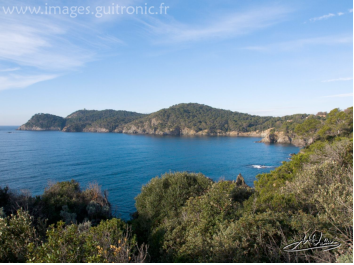
\includegraphics[height=.25\textheight]{Giens}
\caption{Giens sous le soleil}
\label{fig:Giens}
\end{figure}

\subsection{Tableaux}

Pour les tableaux, voir l'exemple Tableau \ref{Tab:tab1}.

\begin{table}[htdp]
\caption{Un exemple de tableau}
\begin{center}
\begin{tabular}{|c|c|c|c|}
\hline
A&1&2&3\\
\hline
B&4&5&6\\
\hline
\end{tabular}
\end{center}
\label{Tab:tab1}
\end{table}%

\subsection{Références bibliographiques}

Les références sont à insérer en fin de document, numérotées par ordre alphabétique des auteurs. Trois exemples de références sont proposés : un article \cite{article} et un acte \cite{acte} et un livre  \cite{livre}.


% ----------------------------------------------------------------------
\begin{thebibliography}{1}
% ----------------------------------------------------------------------
\bibitem{article}
P. Auteur, D. Auteur, T. Auteur. \emph{Titre de l'article}, Revue, Éditeur, page1-pageN, Année. 
\bibitem{acte} P. Auteur. \emph{Titre de l'acte}, Titre de l'ouvrage, Éditeur, page1-pageN, Année.
\bibitem{livre} P. Auteur, D. Auteur. \emph{Titre de l'ouvrage}, Éditeur, Année. 

% ----------------------------------------------------------------------
\end{thebibliography}
% ----------------------------------------------------------------------

% ----------------------------------------------------------------------
\end{document}
% ----------------------------------------------------------------------
